\section*{Implementation}
The program is implemented with \textit{Python 2.7} and the library \textit{Pygame} for the visualization.

\begin{figure}[h]
    \centering
    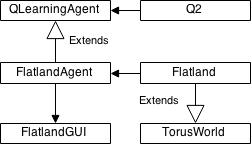
\includegraphics[width=\linewidth]{img/QLearn.png}
    \caption{Main classes and their relations}
\end{figure}

%I went with a modular object-oriented approach for this project.
The class Q2 wraps the data structure for a key-key-value storage.
The class QLearningAgent is an abstract agent that can use Q2
or another Q-class with a different number of keys as it's data structure.
It is inherited by FlatlandAgent which completes the implementation with the problem-specific properties.
The agent stores a Flatland object generated from an input \textit{.txt} and resets this every iteration.
After the desired numbers of iterations the FlatlandGUI class receives the agent
and visualizes it navigating the Flatland.

I also implemented a command line interface that lets the user select a scenario
and set some other paramenters before running a simulation.

~

The algorithm from the project description is implemented in the \texttt{train} method of the QLearningAgent class.
When the agent starts fresh it has no knowledge,
and is forced to make an explorative move.
It then receives an immediate feedback.

If it found poison it receives a large penalty.
If it found food it receives a reward.
If it entered an empty cell it receives a small penalty.
A single step like this will not matter much, but the penalties will accumulate.
This discourages moving back and forth in loops.

When exploring in the beginning the knowledge stored is simply some fraction of the reward or penalty found.
As the agent moves about the world in different iterations it will find itself in situations it has seen before.
The learning then becomes more sophisticated,
taking into account what it knows about a latter state to update the knowledge about a former state.

The Q2 class wraps Python's \texttt{defaultdict} structure,
a key-value storage which returns a default value when the key is non-existant.
Q2 also has utility methods for selecting the best action/value by comparing of the possible values.

~

The \textbf{number of iterations} needed depends on the size of the problem.
This can range from 100 iterations for Flatland number 1 to 10000 for Flatland number 5.

The \textbf{learning rate} and \textbf{discount rate} decide how the knowledge base evolves.
I ended up using a learning rate of $0.3$ and a discount rate of $0.6$ for all the problems.
It is possible that I could have found even better values by testing different combinations more thoroughly and empirically,
but I found these values to work well enough.
A low-ish learning rate means that the agent has to re-test actions a few times to really be sure it is good/bad.
Since eating poison changes the state of the board but not the internal state of the agent,
this is neccessary.
The discount rate must have a diminishing effect,
or else new knowledge could overwrite good knowledge from earlier moves.
This is especially important if a backup scheme is implemented.

The \textbf{backup x} used in $TD(x)$ lets the agent learn "faster", so fewer iterations should be required.
I decided to let this value scale with the size of the Flatland by default,
but it can be specified by the user too.

I also added a \textbf{timeout} (max number of steps),
stopping an agent when it has wandered around the Flatland for too long without finding a solution
and moving on to the next iteration.
This value also grows with the size of the Flatland.

\section*{Selecting actions}
An annealing-inspired temperature variable represents the probability of exploration vs. exploitation,
decreasing linearily with time.
This method is known to handle large solution spaces well,
so it seemed sensible ot use it here.
For each move,
if a random number is below the temperature value, the agent will explore, else it will try to exploit.
If the agent always has the neccesary knowledge,
the ratio of explorative steps should equal the temperature.

Typically a simulation will start with the temperature $1.0$ (but this is configurable).
This is appropriate for the first iteration, since there is no knowledge to exploit anyway.
As the iterations go on the knowledge base grows and the temperature drops.
Ideally it would have the knowledge needed when it rolls for exploitation.
In practice this is not the case all the time, and it will be forced to explore.
So the "experienced temperature",
the actual ratio of exploring moves,
will typically be higher than the temperature variable.
Figure \ref{temp} shows the plot of these two temperatures for 1000 iterations of Flatland number 3,
where a successfull solution was found.

\begin{figure}[t]
    \centering
    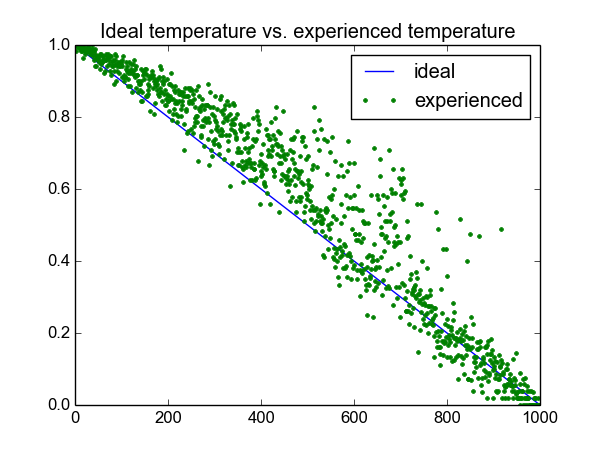
\includegraphics[width=\linewidth]{img/temperature.png}
    \caption{Flatland 3, 1000 iterations}
    \label{temp}
\end{figure}

For most of the run the agent is exploring a great deal more than the ideal temperature would suggest.
The large spread of datapoints in the middle section suggests that the different iterations are diverging
and finding very different states before timing out.
Near the end the values concentrate around the ideal temperature,
suggesting that they are converging on a solution.

\begin{figure}[t]
    \centering
    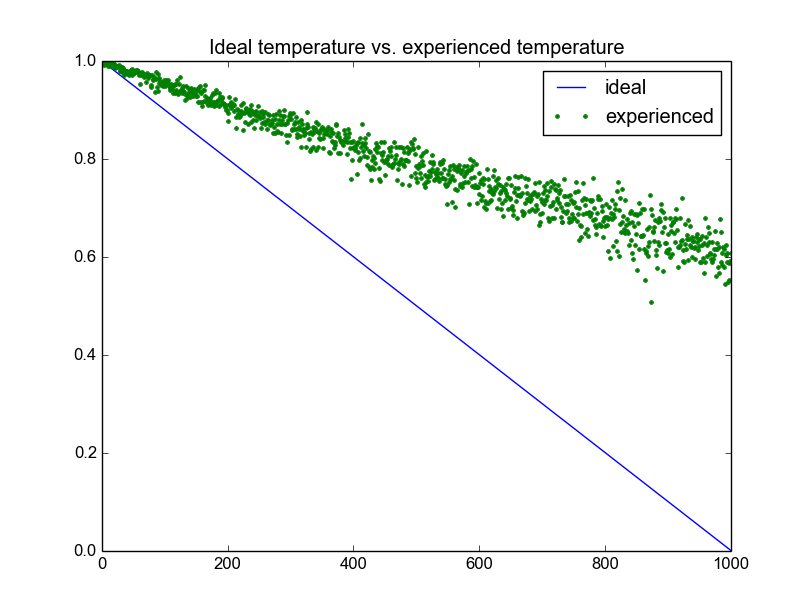
\includegraphics[width=\linewidth]{img/1kFail.png}
    \caption{Flatland 5, 1000}
    \label{fail}
\end{figure}

Figure \ref{fail} shows an attempt to solve Flatland number 5 in just 1000 iterations.
For such a large problem this was not a sufficient number of iterations,
and we can see that the experienced temperature never converges on the ideal temperature.

\section*{Backup scheme}
I started by implementing no backup scheme,
and verified that with sufficient iterations my program was able to solve the problems.

The natural progression from there was to implement $TD(x)$.
I gave the agent a "memory" which would grow to a specified size,
after which adding a new entry would also remove the oldest,
keeping the size fixed.
%Each entry in the memory has a state representation,
%an action, the reward from that action, and the resulting state.
By applying the Q-update procedure starting with the newest memory entry and moving backwards
the knowledge propagates.

With $TD(x)$ I was now able to see that the program could find solutions in fewer iterations.

I was able to see that the common solution found for problem 3, 50 steps, was not the optimal solution.
So I decided to see if I was able to create an implementation of $TD(\lambda)$ that could find a better solution.
This was not successful.
My implementation of $TD(\lambda)$ performed at best the same as the $TD(x)$-implementation at problem 3.
The running time of the program also significantly worsened,
especially noticeable on problems 4 and 5.

I tried for a while to make $TD(\lambda)$ work better, but was not able to, so in the end I reverted back to $TD(x)$.
The final code has no traces of the $TD(\lambda)$ implementation.
